\documentclass[11pt]{article}
\usepackage[sc]{mathpazo} %Like Palatino with extensive math support
\usepackage{fullpage}
\usepackage[authoryear,sectionbib]{natbib}
\linespread{1.7}
\usepackage[utf8]{inputenc}
\usepackage{lineno}
\usepackage{amsmath}
\usepackage{graphicx}
\usepackage{rotating}
\usepackage{longtable}

\usepackage{booktabs}

\begin{document}

\noindent
\textbf{Title}{}: 

\bigskip

\noindent
\textbf{Running title}: Managing a macroparasite: leveraging data and models to mitigate human risk from raccoon roundworm

\bigskip

\noindent
\textbf{Authors}: Sara B. Weinstein$^1$ and Mark Q. Wilber$^2$

\bigskip

\noindent
\textbf{Author affiliations}: \\
1. \\
2. Ecology, Evolution and Marine Biology, University of California, Santa Barbara, Santa Barbara, CA, 93106 \\

\bigskip

\noindent
\textbf{Corresponding author}:

\bigskip

\noindent
\textbf{Word Count}: 

\bigskip

\noindent
\textbf{Keywords}: Individual Based Model, Raccoon, Macroparasite,
Wildlife disease, Zoonosis, Parasite, Management\ldots{}..

\bigskip

\noindent
\textbf{Number of figures}:  \\
\textbf{Article type}: 

\clearpage

\section{Introduction}

Rinderpest is eliminated \citep{Roeder2011}, rabies is reduced \citep{Freuling2013}, and strategies are currently being implemented to manage infectious disease in a number of other wildlife systems [CWD, Koala STDs, etc.]. In many cases, these management strategies have been
guided by mathematical models \citep[e.g.][]{Restif2012,McCallum2017}.  Mathematical models are important when managing wildlife disease because they can be used to both inform to design of field-based management strategies and assess the efficacy of a strategy after implementation  \citep{Restif2012}.  While a number of models have been successfully applied to managing
viral, bacterial and protozoan agents in wildlife populations [give examples, many found in McCallum], models directed
towards managing wildlife macroparasites are still lacking \citep[][, but see X X X for macroparasite models in livestock]{McCallum2017}.

The scarcity of management-based models for macroparasites in wildlife is likely for two reasons. First, macroparasites, such as helminths that do no directly reproduce within a host \citep{AndersonandMay1979}, often have complex life cycles and load-dependent effects on host fecundity and mortality. While these characteristics by no means preclude modeling of macroparasites in wildlife, they do require models that track the distribution of parasite loads across hosts in addition to the total host population and mean parasite load \citep{AndersonandMay1978,Cornell2010}.  These types of models can quickly become challenging to implement, parameterize, and analyze when they are built to ask system-specific questions regarding parasite management in wildlife systems \citep{McCallum2017}.  Second, in contrast the dramatic effects that microparasite epidemics can have on wildlife populations \citep[e.g.][]{Webb2006,Hewson2014} [others], the role of macroparasites as a general regulating factor of wildlife populations is unclear \citep{Tompkins2002,Tompkins2011}. This has potentially led to the perception that detailed macroparasite models in managed wildlife systems are less critical. However, even macroparasites that have equivocal effects on the dynamics of wildlife populations can still be an important concern for human health (Page, Graeff, Kazacos). Therefore, macroparasite models are needed that simultaneously incorporate the macroparasite dynamics in a wildlife reservoir as well as the the risk this reservoir poses to human populations.  

One of the major challenges when using models to manage macroparasite infections in wildlife populations is the scarcity of data.  Collecting individual-based longitudinal parasite intensity data is all but impossible in most wildlife systems due to the difficulty of consistently re-trapping individuals and the fact that accurately measuring parasite intensity often relies on sacrificing a host [citation].  Because of these challenges, the type of data that is often available in wildlife macroparasite systems is cross-sectional age-intensity/prevalence data \citep[i.e. age-intensity/prevalence profiles][]{Pacala1988,Wilson2002}.  An important question in parasite ecology is what can we infer about the host-macroparasite system given an observed age-intensity/prevalence profiles \citep{Pacala1988,Wilson2002,Duerr2003}? With limited prior knowledge about a particular system, the answer is ``not much'' given that multiple mechanisms can lead to very similar age-intensity/prevalence profiles \citep{Wilson2002,Duerr2003}.  However, given some prior knowledge about a host-macroparasite system, this type of data could still be useful for identifying the nature of important components of host-macroparasite systems, such as the structure of transmission.  If this prior knowledge, in the form of an unparameterized dynamic model, can be combined with this type of commonly collected parasitological data, it could aid in the development of empirically parameterized wildlife-macroparasite models that could be used to address questions regarding the management of human exposure risk. 

Because macroparasite models rely on individual-based models to capture the complexities of parasite load heterogeneity, age-structure, and concomitant immunity \citep[e.g.][]{Cornell2005,Drawert2017,McCallum2017} [OTHERS], linking unparameterized macroparasite models with empirically observed age-intensity/prevalence profiles is challenging.  Often these models do not have easily defined likelihood functions, such that standard likelihood-based fitting techniques can not be used. One alternative approach for fitting individual-based models to age-intensity/prevalence data is Approximate Bayesian Computing (ABC) \citep{Beaumont2010}. ABC substitutes the likelihood function with a user-defined distance function and then tries to identify a set of model parameters that minimizes the distance between an observed pattern (e.g. the observed age-intensity/prevalence profile) and the same pattern generated by the model for a given set of parameters (e.g. a simulated age-intensity/prevalence profile) \citep{Toni2009,Beaumont2010}.  The ABC method has been successfully applied in host-microparasite systems to estimate transmission dynamics from observed data \citep{Conlan2012,Kosmala2015}, yet its ability for identifying the structure of parasite transmission has not yet been demonstrated in macroparasite systems using commonly collected age-intensity/prevalence data. 

We fill this knowledge gap by developing an individual-based model for the macroparasite raccoon roundworm \emph{Baylisascaris procyonis}. Raccoon roundworm is recognized as a threat to both human and wildlife health \citep{Page2011,Weinstein2017} and is difficult to control due to its complex life cycle
and resistant environmental infectious stages. Worms mature in the
raccoon gut and infected raccoons can release over a million parasite
eggs per day [citation]. Eggs survive for over a year (Shafir) and accumulate at
communal raccoon defecation sites termed latrines [citation]. Individual
raccoons contribute to multiple latrines and these contaminated sites
expose raccoons and other species to eggs. Eggs infect juvenile
raccoons, leading to high parasite loads in animals as young as four
months \citep{Weinstein2016} [TODO: Fill in these citations: Kazacos, Boyce]. Raccoon susceptibility to eggs
declines with age and adult raccoons acquire worms by eating infected
small mammals and birds [citation]. In these birds and mammals, larval worms do
not mature. Instead, larval worms migrate from the gut into other
tissues including the brain, often causing fatal neurological damage.
Raccoons scavenge these incapacitated animals [citation], and this trophic
transmission maintains infection in older raccoons that are less
susceptible to eggs [citation]. Nearly all infected raccoons release eggs;
however higher parasite loads in juveniles suggests that this age class
contributes disproportionately to human disease risk [citation].

Using this individual-based model, we perform simulations to understand the conditions under which known transmission parameters can be recovered from age-intensity/prevalence data using the ABC approach.  We then fit the individual-based model to observed age-intensity/prevelance data and used the resulting model to explore the efficacy of various management strategies for reducing human risk to \emph{Baylisascaris procyonis} exposure. This work demonstrates that given some prior knowledge of a host-macroparasite system reflected in the form of a dynamic model, age-intensity/prevalence data can be used to infer unknown parameters in the transmission function. Moreover, we use this approach to demonstrate that it is largely ineffective to reduce human risk to raccoon roundworm via strategies such as culling, deworming, and birth control. Rather, we found that the only effective management strategy was reducing the environmental pool of parasites via cleaning-up raccoon latrines. 




% The macroparasite raccoon roundworm \emph{Baylisascaris procyonis} is increasingly recognized as a threat to both human
% and wildlife health \citep{Page2011,Weinstein2017}, but, like many
% macroparasites, is difficult to control due to its complex life cycle
% and resistant environmental infectious stages. Worms mature in the{}
% raccoon gut and infected raccoons can release over a million parasite
% eggs per day [citation]. Eggs survive for over a year (Shafir) and accumulate at
% communal raccoon defecation sites termed latrines [citation]. Individual
% raccoons contribute to multiple latrines and these contaminated sites
% expose raccoons and other species to eggs. Eggs infect juvenile
% raccoons, leading to high parasite loads in animals as young as four
% months \citep{Weinstein2016} [TODO: Fill in these citations: Kazacos, Boyce]. Raccoon susceptibility to eggs
% declines with age and adult raccoons acquire worms by eating infected
% small mammals and birds [citation]. In these birds and mammals, larval worms do
% not mature. Instead, larval worms migrate from the gut into other
% tissues including the brain, often causing fatal neurological damage.
% Raccoons scavenge these incapacitated animals [citation], and this trophic
% transmission maintains infection in older raccoons that are less
% susceptible to eggs [citation]. Nearly all infected raccoons release eggs;
% however higher parasite loads in juveniles suggests that this age class
% contributes disproportionately to human disease risk [citation].

% Human risk might be reduced by removing \emph{B. procyonis} eggs from
% the environment, treating infected raccoons, or reducing raccoon
% populations. Culling is often considered as a possible control
% disease control strategy \citep{Wasserberg2009,Langwig2015}. However, although a common component of
% rabies control \citep{Rosatte1986}, culling is controversial and not
% always effective \citep{Choisy2006a,Beeton2011,Morters2013}. Birth control is a less controversial method to
% reduce wildlife populations \citep{Smith2002a}, but is often slower, more
% expensive, and less effective than culling (citations). As an alternative to
% reducing host populations, parasite populations can be reduced through
% mass drug administration (Qureshi 1994 et al, deer fascioloides) or
% vaccination (anthrax antelope De vos 1973 Koedoe, bison; elk brucellosis
% (rabies). Although no \emph{Baylisascaris} vaccines exist, the mass
% baiting methods developed for rabies vaccines can also deliver deworming
% medication (anthelminthics) \citep{Smyser2015} [What about Smyser 2013?]. These anthelminthic
% baits can reduce \emph{B. procyonis} prevalence in wild raccoons, but
% raccoons are rapidly re-infected unless latrines are also removed \citep{Page2011} [citation for Page et al. 2014?]. Latrine, parasite, and raccoon removal
% all could reduce human \emph{B. procyonis} exposure; however,
% experiments that compare these strategies are difficult to implement in
% wild animal populations.

% In this study we use a combination of previously published results, field estimated parameters, and model fitting approaches to parameterize an individual-based model of raccoon roundworm.  In this model, we track both the proximity of raccoons to human habitation as well as the within-host dynamics of raccoon roundworm. We then use this model to investigate how different management strategies affect \emph{B. procyonis} populations, raccoon populations, and human risk of infection. We find that managing human risk to raccoon roundworm via strategies such as culling, deworming, and birth control were largely ineffective for mitigating human risk. Instead, the only effective management strategy was reducing the environmental pool of parasites via cleaning latrines. 

\section{Methods}

The methods are broken into three section.  First, we provide an overview and justification of the individual-based model that we built to explore the dynamics of \emph{B. procyonis} in raccoon populations. Second, we describe how we used this model to test the ability and limitations for inferring transmission dynamics from age-intensity/prevalence data using the ABC method. Finally, after fitting this model to an empirically observed age-intensity/prevalence profile in raccoon roundworm, we describe how we implemented different potential management strategies for raccoon roundworm.

\subsection{Description of the individual-based model}

To evaluate raccoon roundworm management strategies, we built an
individual-based model for a macroparasite with long-live
environmental infectious stages and complex life cycle. We describe this
model using the Overview, Design concepts, Details (ODD) protocol \citep{Grimm2006,Grimm2010}, providing first an Overview of the model, then
describing the Design Concepts, followed by the Details of submodels,
parameterization and initialization. Additional details on submodels and
annotated code are available in the Supplementary Material.

\subsection{Overview}

\subsubsection{Purpose}

We developed an individual-based macroparasite model for raccoon and
raccoon roundworm to compare how host, parasite, and infective stage
targeted management affect host demography, parasite demography and
human exposure.

\subsubsection{Entities, state variables, and scales}

In this model, raccoons are the main model entity and exist as an age
structured, closed, all-female population. Five attributes describe each raccoon: an identification number, an age, an alive
or dead status, a location and a parasite load. We track the female parasite
load (i.e. the infrapopulation) within each raccoon. Raccoons can acquire new
worms at each time step and, for every raccoon, we explicitly track the age of each
worm cohort. Worms accumulate and die over time, and we
calculate parasite load by summing across parasite cohorts within each raccoon.
Infected raccoons contaminate the environment with long-lived parasite
eggs, which we model as an environmental egg pool. As even a single worm
can produce more than a million eggs per month [citation], we assume that infected
raccoons rapidly saturate local latrines with eggs. Thus, we do not
explicitly track each egg, and instead use infection prevalence in the
local raccoon population as a proxy for local egg production. Eggs decay
over time () and we calculate the current environmental egg pool as a
weighted sum of past egg production. Eggs also infect rodents that co-occur with raccoons. We use the
environmental egg pool to estimate rodent infection at each time step. [However, because \emph{B. procyonis} is not reproductive in rodents, infected rodents do not directly contribute to the environmental egg pool.]

We track hosts, parasites, and environmental egg pools in a spatially
implicit 20 km\textsuperscript{2} world with ten equally sized two
km\textsuperscript{2} zones. Human population density increases
consecutively from zones one through ten (Fig X, x) and zones with
higher human density support larger raccoon populations (citation, Fig. X). 

% We track the
% raccoon population, parasite population, and egg pool in each zone at
% monthly time steps for 400 months, using the egg pool in each zone to
% calculate total human risk within the simulated world.

\subsubsection{Process overview and scheduling}

We update the model on a monthly time step. The first event that occurs in a time step is raccoon survival. Surviving raccoons then reproduce, lose
parasites, gain parasites, disperse, age, and contribute to the
environmental egg pool. Following the typical raccoon life cycle,
raccoons reproduce once per year, with kits entering the population in
the following time step. All other events occur monthly in all ten
zones.

\subsection{Design Concepts}

\subsubsection{Emergence and Interactions}

Although some infectious agents can regulate their hosts (), raccoon
roundworm does not regulate raccoons [citations]. Unmanaged raccoon populations are
limited by resource availability (), which we model by setting a raccoon
carrying capacity in each zone. As raccoon population density
increases within a zone, reproduction declines following a Ricker function \citep{Gurney1998}. Simulated raccoons
reproduce once per year (in the spring), and this pulsed reproduction
produces realistic annual population cycles and age distributions for an
unmanaged raccoon population (gehrt, others).

We add macroparasites to this simulated raccoon population following
classic macroparasite modeling theory \citep{AndersonandMay1978,Anderson1991,Cornell2010}. Individual host-parasite interactions generate an aggregated
parasite population with realistic age-intensity and age-prevalence
profiles. The parasite population cycles due to
changing host demography, and these emergent patterns match the widely
observed fall rise in mean raccoon parasite loads (eg page 2016,
weinstein2016, many others).

\subsubsection{Stochasticity}

We determine the following modeling events using a random number generator in R version 3.2.4: raccoon survival, raccoon reproduction, raccoon litter size, raccoon dispersal, parasite loss, and parasite gain.  The probability of a particular realization of any of these events depends on the biology of the raccoon-\emph{B. procyonis} described in \emph{Submodels}.

\subsubsection{Initialization}

We began each simulation with 500 two-year old raccoons stochastically
distributed throughout the 20 km$^2$ world according to
zone specific carrying capacities. The average starting zone densities from lowest to highest were 1.58, 12.32, 27.56, 40.68, 52.84, 61.84, 69.74, 74.52, 77.18, and 81.74 raccoons per two km$^2$.
Initially, each raccoon hosted 10 worms and no eggs contaminated any
zones. The mean rodent worm load was initially 3.49 based on
empirical observations (Weinstein, unpublished) and the variance of rodent worms
was set to 87.08 based on the canonical scaling relationship between
log-mean parasite load and log-variance in parasite load \citep{Shaw1995}.

\subsection{Submodels}

\subsubsection{Raccoon death}

We assume that all raccoons experience a constant per month death
probability and then augment this age-independent death rate to account
for high nestling mortality (Montgomery 1969) and senescence. Nestling
raccoons (\textless{}1 month) have constant added risk of death and we
model senescence as an increasing age-specific hazard rate,
parameterized to ensure that raccoons cannot live past 20 years old [citation].
These three mortality processes lead to a ``bathtub''-shaped hazard
function for raccoon mortality (Fig. \ref{fig:mod_diagram})

Raccoons can also die from \emph{B. procyonis} infection if worms cause
an intestinal obstruction (Stone, 1983; Carlson and Nielsen, 1984).
Fatal obstructions can occur at loads as low as 141 worms and have been
recorded in animals with 636 and 1,321 worms (Stone, 1983; Carlson and
Nielsen, 1984), however raccoons can survive with over 200 worms
(Kazacos 2001). To model this potential parasite-induced host mortality,
we use a logistic parasite-induced mortality function
\(1 - \frac{e^{\beta + \alpha*log(load + 1)}}{1 + e^{\beta + \alpha*log(load + 1)}}\)
, where $\alpha$ gives the per parasite effect on the log
odds raccoon survival probability over a month and $\beta$ relates to the threshold at which parasite-induced mortality begins
to occur \citep{Wilber2016}. We estimated these parameters using... Our parameterization corresponds with the empirical observation that parasite-induced mortality is not a large factor affecting raccoon dynamics.

\subsubsection{Raccoon reproduction}

Raccoons typically reproduce once a year and can have up to 2 female
young per litter (Gehrt 2001, Fritzell 1985, Cowan 1973, clark et al
1989). Although there is some evidence that populations in the far south
of the range may breed year round (Troyer et al 2014) and late litters
do occur (Gehrt and Fritzell 1996, 1978a?), here we assume that all
reproduction occurs in a single spring pulse (Fig. \ref{fig:mod_diagram}).

The model assumes that average raccoon litter size in a given year
decreases with increasing raccoon density (Fig. \ref{fig:mod_diagram}). This density-dependence
corresponds with reproduction in dense populations being limited by both
the availability of nest sites and increased infanticide risk in dense
populations (Gehrt and Fritzell 1999; hauver 2010; Wolff 1997).
Specifically, we model this density-dependence following a Ricker
function (Table X).

Raccoons kits are born into the same human overlap zone as their mothers and stay with their mothers for about a year (citation).  After a year, juvenile raccoons disperse to a new zone. We modeled the probability of a juvenile raccoon dispersing to any particular zone (including the zone in which they were born) being proportional to the ratio between the carrying capacity of that zone and the current density of the zone. This means that juvenile raccoons were more likely to disperse to zones that had less raccoons relative to the zones carrying capacity [TODO: CHECK THE IMPLEMENATION OF THIS].  Once a juvenile disperses to a new zone, we assumed that it remained in this zone for the rest of its life. 

\subsubsection{Worm transmission}

Raccoons acquire \emph{B. procyonis} through two transmission routes:
encounter with \emph{B. procyonis} eggs in the environment and by
consuming other animals already infected with \emph{B. procyonis} adults
(e.g. rodents) (citations).  We assume that raccoons encounter eggs with some probability that is proportional to the total number of eggs in the environment. Raccoons only encounter eggs in the zone that they occupy. Conditional on encountering eggs, the total number of eggs encountered follows a negative binomial distribution with a fixed aggregation parameter and fixed number of mean eggs encountered.  Finally, the probability that any one of these eggs actually infects the raccoon is a decreasing function of how infected the raccoon (i.e. increased load decreases susceptibility) and is zero if the raccoon is older than 4 months (citations). Finally, the worms are acquired from rodents if the raccoon is older than 4 months.  Rodents are encountered and consumed with some probability and the number of worms in the rodent follows a negative binomial distribution with the mean that has a maximum value of 3.49 worms per mouse and decreases with decreasing environmental egg pool. As stated above, variance scales with the mean according to Taylor's Power Law \citep{Shaw1995}.  The aggregation parameter and mean parameter when encountering eggs in the environment, the parameter the determines how encounter probability scales with the size of the environmental egg pool, and the rodent encounter probability are all unknown for this system and needed to be estimated using age-intensity/prevalence data estimated and the ABC method.

\subsubsection{Worm death}

Worms die according to an age-dependent survival function that follows the logistic curve $\frac{1}{\exp(-(a + b \text{age})}$ (Fig. \ref{fig:mod_diagram}) [DEFINE THIS CONSISTENTLY]. This function was parameterized with data from Olsen 1958 [Sara, more detail about this study here].  Note that we do not include any negative density-dependence in parasite death rate as we instead included this density-dependence in the probability of a worm successfully establishing (see \emph{Worm transmission}).

\subsection{Inferring susceptibility and transmission parameters with ABC-SMC}

\subsubsection{Simulating age-intensity/prevalence profiles}

As shown in Table 1, the raccoon IBM had four parameters relating to susceptibility and transmission that were unknown: 
the mean number of eggs encountered by a raccoon in the environment over
a monthly time step, the variability in the number of eggs encountered
over a monthly time step, an egg encounter parameter relating the eggs
in the environment to the probability of a raccoon encountering an egg, and
the probability of a raccoon consuming a rodent in a month.

Using our model, we explored whether commonly collected age-intensity/prevalence profiles contained enough information to estimate these unknown parameters.  In particular, we considered a set of known susceptibility and transmission parameters that produced age-intensity/prevalence profiles generally consistent with what we saw in raccoon-\emph{B. procyonis} systems (Fig. X).  With these known parameters, we then simulated the raccoon IBM until it was stationary and then sampled 189 raccoons according to the age-structure given in \cite{Weinstein2016}.  Using these simulated and sampled raccoons, we built an age-intensity/prevalence profile that we considered our ``\emph{in silico} observed'' data (as opposed to the ``empirically observed'' data given by \cite{Weinstein2016}).

\subsubsection{The ABC-SMC method}

Given our ``\emph{in silico} observed'' data, we then tested whether we could recover the known susceptibility and transmission parameters using Approximate Bayesian Computing
with Sequential Monte Carlo (ABC-SMC) \citep{Sisson2009,Toni2009,Beaumont2010,Kosmala2015}. ABC is a likelihood-free parameter estimation method and is often used with simulation-based
models in which the likelihood of data given the model is
intractable to compute. Instead, ABC uses a user-defined distance
function to determine how ``well'' the simulation model parameterized
with a set of parameters drawn from some prior distribution can
reproduce the observed data. This approach allows one to estimate an
approximate posterior distribution for unknown parameters in a model based
on how well they can reproduce observed data.  Moreover, it shows which parameters in the model are identifiable  from the data provided \citep{Toni2009}.

The ABC-SMC algorithm we used is as follows \citep{Toni2009,Sisson2009,Beaumont2010}

\begin{enumerate}
\def\labelenumi{\arabic{enumi}.}
\item
  We specified uniform priors around our four unknown transmission and
  susceptibility parameters: $\mu_{\text{encounter}} \sim \text{Uniform}(10, 1000)$, $k'_{\text{encounter}} = \frac{1}{1 + k_{\text{encounter}}} \sim \text{Uniform}(0, 1)$, $\text{egg encounter} \sim \text{Uniform}(0.001, 5)$, and $p_{\text{rodent encounter}} \sim \text{Uniform}(0, 1)$.
\item
  We drew 10,000 samples from each prior distribution such that we had
  10,000 vectors of parameters (henceforth a parameter vector is called a particle).
\item
  For each of the 10,000 particles, we simulated our model for 100
  months to remove the effects of the initial conditions.
\item
  For a given simulation, we then sampled 189 raccoons over the last 24
  months of the simulation, consistent with how we sampled the ``observed'' data.
\item
  Using this sample, we then constructed the age-intensity/prevalence
  profile from the simulated data and compared it to the ``observed'' age-
  abundance/prevalence.
\item
  To compare the simulated and observed data, we first combined the
  eight observed age-intensity data points, the eight observed interquartile ranges for the age-intensity data points, and the eight observed
  age-prevalence data points into a vector S$_\text{obs}$ = [age-intensity$_1$,
  age-intensity$_2$, \ldots{}, age-intensity$_8$, iqr$_1$, iqr$_2$, \ldots{}, iqr$_8$, age-prev$_1$,
  age-prev$_2$, \ldots{}, age-prev$_8$]. We did the same thing for all
  10,000 simulated age-abundance/prevalence profiles such that we had a
  10,000 x 24 matrix (S$_\text{sim}$) where the columns matched the 24 dimensions
  in S$_\text{obs}$ and the rows corresponded to one of the randomly drawn
  particles.
\item
  To put the intensity data, IQR data, and prevalence data on the same
  scale, we standardized each column in S$_\text{sim}$ by subtracting the mean
  and dividing by the standard deviation of each column. We then
  performed this identical transformation on S$_\text{obs}$ \emph{based on the
  column-wise means and standard deviations from S$_\text{sim}$}. This
  transformation of S$_\text{obs}$ put the values of S$_\text{obs}$ in terms of
  deviations relative to the mean of the simulated data.
\item
  We then calculated the Euclidean distance between each row in S$_\text{sim}$
  and S$_\text{obs}$ (i.e. the L2 norm), which resulted in 10,000 distance
  measures. We then accepted the 500 particles that resulted in the
  500 smallest distances.
\item
  We then equally weighted each of these 500 accepted particles and
  resampled them with replacement 10,000 times. Upon sampling a
  particle, we perturbed each parameter in a particle by
 $\sigma_i \text{Uniform}(-1, 1)$ where $\sigma_i$ is the standard
  deviation of the $i$th parameter in the 500 accepted parameters. This
  perturbation helps the algorithm explore nearby parameter space. If this perturbation pushed any parameter inside a particle outside of the range of its prior distribution, we set the new particle equal to the old particle without perturbation [POTENTIALLY IMPLEMENT DIFFERENTLY].
\item
  We then repeated 3 - 9 with the 10,000 perturbed parameters 5
  times with one important change to step 9 after the first round of
  sampling. After identifying 500 accepted particles we used the
  following function to weight each particle \citep{Toni2009}

  \begin{equation}
    w_t^{(i)} = \dfrac{\pi(\theta_t^{(i)})}{\sum_{j = 1}^N w_{t - 1}^{(j)} K_t(\theta_{t - 1}^{(j)}, \theta_t^{(i)})}
  \end{equation}

  where $\theta_i$ refers to particle $i$, $t$ refers to the $t$th iteration greater with $t > 1$,  $K_t(\theta_{t - 1}^{(j)}, \theta_t^{(i)})$ is probability of the current particle based on the previous particle and the perturbation kernel $K_t$. 
  In summary, this is the
  importance weighting of a particle that accounts for the fact that
  particles are no longer being sampled from the prior distribution \citep{Beaumont2010}.
\end{enumerate}

We applied the ABC-SMC method to the ``\emph{in silico} observed'' age-intensity/prevalence data and obtained posterior distributions for the four [MAYBE FIVE?]
transmission and susceptibility parameters in the raccoon-\emph{B.
procyonis} model.  We also varied the type of data that we were passing into ABC-SMC method to explore how different aspects of the age-intensity/prevalence profile affected our ability to estimate the transmission and susceptibility parameters.  In particular, we tried estimating the parameters with only mean intensities across age groups, only prevalences across age groups, both mean intensities and prevalences, and mean intensities, prevalences, and IQRs. 

For each different ABC run, we then examined the marginal posterior distributions of each parameter to determine which of these parameters were inferable from the age-intensity/prevalence data and whether the known parameters could be recovered with any precision. Finally, we performed posterior predictive diagnostics and compared the simulated age-intensity/prevalence profiles from the estimated posterior distributions to the ``\emph{in silico} observed'' data.

Finally, after identifying the successes and limitations of the inferring known transmission and susceptibility parameters from simulated age-intensity/prevalence data, we applied the ABC-SMC algorithm discussed above to the empirically observed age-intensity/prevalence data in the raccoon-\emph{B. procyonis} system. [Also tested different assumptions about concomitant immunity?]

% Before applying this algorithm to the empirical raccoon-\emph{B. procyonis} data, we tested the ability of this algorithm to recover known transmission parameters from age-intensity/prevalence data.  To do this, we fixed the four parameters of interest at specific, known values and simulated the raccoon IBM for 100 years (Supplementary Material).  We then sampled 189 raccoons present over the last two years of the model with the same age-structure as given in \cite{Weinstein2016} and considered this our ``observed \emph{in silico}'' data.  We then ran the ABC-SMC algorithm using this ``observed \emph{in silico}'' data and found that we could recover the true mean number of eggs encountered, the variability in eggs encountered, and the probability of encountering a rodent with some specificity, but could not reliably recover the egg contact parameter [WC] (see Supplementary Material). [Post-hoc simulation analyses illustrated that this parameter has little influence on the resulting age-intensity/age-prevalence profiles, which is consistent with the ABC-SMC algorithm not being able to identify it (Supplementary Material).] With this caveat in mind, we applied the ABC-SMC algorithm to the observed age-intensity/prevalence data from \cite{Weinstein2016}.

\subsection{Management strategies for \emph{B. procyonis}}

We used our fully parameterized model to explore how different
management strategies affected the dynamics of worm and raccoon
populations and human risk of encounter with \emph{B. procyonis}. We considered four
distinct management strategies in addition to combinations of these
management strategies: culling raccoons, birth control of raccoons,
anti-helmenthic baiting, and latrine cleanup. For each of these
management strategies, we considered different levels of management
effort (see below for definitions) and explored how different management
strategy-by-effort combinations affected four major predictions of the
model: the total raccoon population, the total worm population, the level of human risk, adn the mean raccoon worm load

For each management strategy, the model was run for 200 months to
obtain equilibrium dynamics, at which time the management strategy was
enacted monthly for an additional 200 months (FIG. X). Upon completion
of the simulation, the four major model predictions listed above were
computed based on the mean value over the last 24 months of the simulations.

The different biological basis of the management strategies and there implementation in the model are described below

\bigskip
\noindent
\emph{Culling raccoons}

Culling is a commonly discussed management strategy for wildlife disease. [SARA: Could you add a paragraph on culling?]

To implement raccoon culling, we assumed that some number of traps were
randomly distributed in the raccoon world each month. We assumed that
per trap probability of catching a raccoon increased with raccoon
density following a type I functional response: $1 - \exp(-\text{raccoon
density} \gamma)$. $\gamma$ was estimated
based raccoon trapping data from  Prange et al. (2003) and Graser et al.
(2012) (probably more description here\ldots{} in the Sup Material). Finally, we assumed
that the number of raccoons were caught each month (\texttt{num\_trapped}) followed a Binomial distribution with parameters $N$ = the number of traps deployed that month and $p$ = per trap probability of catching a raccoon as described above. Because we assumed that all
individual raccoons were equally likely to be trapped, we then randomly
selected \texttt{num\_trapped} raccoons from the
population to cull in that time step.

We also allowed trapping to occur in specific zones of human overlap and
only for particular age raccoons. When trapping in a particular zone(s)
of human overlap, trapping probability was determined only by the
density of raccoons in that zone(s) and only raccoons in that zone could
be trapped and culled. When trapping for a particular target age class,
trapping proceeded as described above, but raccoons that were not in the
target age class were released.

\bigskip
\noindent
\emph{Birth Control}

[SARA: Could you add a few sentences on birth control]

Birth control followed the exact same trapping regime as culling.
However, upon trapping a raccoon it was no longer able to reproduce for the remainder of its life. However, this raccoon could still be trapped again in proceeding months. 

\bigskip
\noindent
\emph{Anti-helminthic baiting}

[SARA: Could you add some information on anti-helminthic baiting]

We implemented anti-helminthic baiting by first randomly distributing
some number of baits into the raccoon world. Of the initial number of
baits distributed into the world, on average 60\% of these
baits were degraded or consumed by animals other than raccoons [citations]. For the
remaining baits, we assumed that all raccoons were equally likely to
consume a bait and randomly assigned baits to raccoons in the world. A
given raccoon could consume multiple baits in a month. Upon consuming a
bait, all the worms in a raccoon were killed, but the raccoon could
immediately start acquiring worms again from the environment and
rodents. Consuming one bait or multiple baits in a month had identical
effects on raccoon worm loads. Similar to culling and birth control, we
also allowed for anti-helminthic baiting in specific zones of human
overlap.

\bigskip
\noindent
\emph{Latrine cleanup}

[SARA: Could you add some background information]

The final management strategy we explored was latrine cleanup. This strategy was implemented by reducing or
eliminating the environmental egg pool each month.  By reducing or eliminating the egg pool, this strategy directly affected the risk of human infection as humans obtain infections through eggs in the environment.  Therefore, we would \emph{a priori} expect this strategy to be effective.  However, our expectations are less clear regarding the efficacy of the aforementioned strategies compared to latrine cleanup. Similar to the other strategies, latrine cleanup could be specifically implemented in particular zones of human overlap as each zone has its own independent egg pool. 

\section{Results}

\subsection{Inferring transmission and susceptibility parameters from age-intensity/prevalence data}

\subsubsection{Simulated data}

Using simulated age-intensity/prevalence profiles (Fig. X) as our ``\emph{in silico} observed'' data, we explored the ability of this type of data combined with the ABC-SMC method to recover known transmission and susceptibility parameters.  Given the age-intensity, -prevalence, and -IQR data, we were able to recover three of our four transmission and susceptibility parameters: the probability of encountering and rodent, the mean number of eggs encountered per month by a raccoon, and the variability in the number of eggs encountered. The posterior distributions of these three parameters were all significantly different than the prior distributions and the true values used to simulate the data were contained in the approximate 95\% credible intervals of the posterior distributions.  [Discuss the size of the intervals]. However, we were unable to infer the contact parameter from the age-intensity/prevalence data. Additional simulations indicated that this was because the environmental egg pool was so large that egg contact was almost guaranteed regardless of the exact value of this parameter [CHECK].  In other words, the age-intensity/prevalence profile was not sensitive to deviations in the the contact parameter as it was thus not inferable from the data.

Posterior predictive simulations [check terminology] showed that the posterior distributions of the unknown parameters were able to generate age-intensity/prevalence profiles consistent with the ``\emph{in silico} observed'' data. 

When we only used pieces of the age-intensity/prevalence profile to fit the unknown transmission and susceptibility parameters, we lost the ability to estimate other transmission and susceptibility parameters it a fairly intuitive way. For example, when we only used the prevalence data, we were no longer able to infer the mean number of contact.  Also, when we did not include IQR, we lost the ability of to estimate the variability in the number of eggs acquired per contact. [TODO adjust as necessary]

\subsubsection{Empirical data}




\subsection{Managing human risk to \emph{B. procyonis} exposure}

\section{Discussion}

Major talking points in the discussion

1. Modeling macroparasites in wildlife and leveraging the data at hand
2. Our study shows that with some prior information in the form of a dynamic model is available, age-intensity/prevalence profiles can be used to test hypotheses about the transmission and susceptibility of hosts.
3. This really useful because this is the type of data that is often collected in wildlife parasite systems so our approach is widely applicable to other wildlife-macroparasite systems (note that it has already been applied to microparasite systems with success)
4. We used the information gained about transmission and susceptibility to explore the efficacy of potential management strategies for raccoon round worm. 
5. Because eggs are distributed in the environment

When we talk about birth control- There is currently no approved raccoon
contraceptive (), although products developed for dogs and cats could be
optimized for raccoons given high cost and not great results, strategy
doesn't seem worth pursuing.

Culling- potential for a ``Hydra effect'': It's got a name! Abrams 2009.
When does greater mortality increase population size? the long history
and diverse mechanisms underlying the hydra effect. Ecology Letters
12:462--474 (named for greek myth, where chopping of one hydra head
caused two to grow back. While density dependent birth rates set up
possibility, and do lead to increased prev/intensity in animals, overall
reduction in rac population still reduces human risk, although not as
quickly perhaps as would if no ``hydra effect'' occurred.

\section{Acknowledgments} 

Acknowledgments, including funding
information, should appear in a brief statement at the end of the body
of the text. Acknowledgments of specific author contributions to the
paper should appear here.

% \textbf{Literature cited}

% Braae, U. C., B. Devleesschauwer, S. Gabriël, P. Dorny, N. Speybroeck,
% P. Magnussen, P. Torgerson, and M. V. Johansen. 2016. CystiSim -- An
% agent-based model for \emph{Taenia solium} transmission and control.
% PLoS Negl Trop Dis \textbf{10:} e0005184.

% Choisy, M., and P. Rohani. 2006. Harvesting can increase severity of
% wildlife disease epidemics. Proceedings of the Royal Society B:
% Biological Sciences \textbf{273:} 2025-2034.

% Elmore, S. A., R. B. Chipman, D. Slate, K. P. Huyvaert, K. C.
% VerCauteren, and A. T. Gilbert. 2017. Management and modeling approaches
% for controlling raccoon rabies: The road to elimination. PLoS Negl Trop
% Dis \textbf{11:} e0005249.

% Graeff-Teixeira, C., A. L. Morassutti, and K. R. Kazacos. 2016. Update
% on baylisascariasis, a highly pathogenic zoonotic infection. Clinical
% Microbiology Reviews \textbf{29:} 375-399.

% Kazacos, K. R. 2001. \emph{Baylisascaris procyonis} and related species.
% \emph{In} Parasitic Diseases of Wild Mammals W. M. Samuel, M. J. Pybus,
% and A. A. Kocan (eds.). Iowa State University Press, Ames, Iowa, p.
% 301-341.

% Kazacos, K. R. 2016. \emph{Baylisascaris} larva migrans. Vol. 1412 p.
% 1-122. U.S. Geological Survey Circular: 1412, Reston, Viriginia.

% Morters, M. K., O. Restif, K. Hampson, S. Cleaveland, J. L. N. Wood, and
% A. J. K. Conlan. 2013. Evidence-based control of canine rabies: a
% critical review of population density reduction. Journal of Animal
% Ecology \textbf{82:} 6-14.

% Page, K., J. C. Beasley, Z. H. Olson, T. J. Smyser, M. Downey, K. F.
% Kellner, S. E. McCord, T. S. Egan, 2nd, and O. E. Rhodes, Jr. 2011.
% Reducing \emph{Baylisascaris procyonis} roundworm larvae in raccoon
% latrines. Emerging Infectious Diseases \textbf{17:} 90-93.

% Page, K., T. J. Smyser, E. Dunkerton, E. Gavard, B. Larkin, and S.
% Gehrt. 2014. Reduction of \emph{Baylisascaris procyonis} eggs in raccoon
% latrines, suburban Chicago, Illinois, USA. Emerging Infectious Diseases
% \textbf{20:} 2137-2140.

% Page, K. L. 2013. Parasites and the conservation of small populations:
% The case of Baylisascaris procyonis. International Journal for
% Parasitology: Parasites and Wildlife \textbf{2:} 203-210.

% Rosatte, R. C., M. J. Pybus, and J. R. Gunson. 1986. Population
% reduction as a factor in the control of skunk rabies in Alberta. Journal
% of Wildlife Diseases \textbf{22:} 459-467.

% Sircar, A. D., F. Abanyie, D. Blumberg, P. Chin-Hong, K. S. Coulter, D.
% Cunningham, W. C. Huskins, C. Langelier, M. Reid, B. J. Scott, D.-A.
% Shirley, J. M. Babik, A. Belova, S. G. H. Sapp, I. McAuliffe, H. N.
% Rivera, M. J. Yabsley, and S. P. Montgomery. 2016. Raccoon roundworm
% infection associated with central nervous system disease and ocular
% disease---six states, 2013--2015. Morbidity and Mortality Weekly Report
% \textbf{65:} 930-933.

% Smyser, T. J., S. R. Johnson, M. D. Stallard, A. K. McGrew, L. K. Page,
% N. Crider, L. R. Ballweber, R. K. Swihart, and K. C. VerCauteren. 2015.
% Evaluation of anthelmintic fishmeal polymer baits for the control of
% \emph{Baylisascaris procyonis} in free-ranging raccoons (\emph{Procyon
% lotor}). Journal of Wildlife Diseases \textbf{51:} 640-650.

% Sterner, R. T., M. I. Meltzer, S. A. Shwiff, and D. Slate. 2009. Tactics
% and economics of wildlife oral rabies vaccination, Canada and the United
% States. Emerging Infectious Diseases \textbf{15:} 1176.

% Woodroffe, R., C. A. Donnelly, H. E. Jenkins, W. T. Johnston, D. R. Cox,
% F. J. Bourne, C. L. Cheeseman, R. J. Delahay, R. S. Clifton-Hadley, G.
% Gettinby, P. Gilks, R. G. Hewinson, J. P. McInerney, and W. I. Morrison.
% 2006. Culling and cattle controls influence tuberculosis risk for
% badgers. Proceedings of the National Academy of Sciences \textbf{103:}
% 14713-14717.



\bibliographystyle{/Users/mqwilber/Dropbox/Documents/Bibformats/ecology.bst}
\bibliography{/Users/mqwilber/Dropbox/Documents/Bibfiles/Projects_and_Permits-raccoon_IBM.bib}

\clearpage

\linespread{1}
\scriptsize
\renewcommand{\arraystretch}{1.2}
\begin{longtable}{p{4.5cm} p{4.5cm} p{5cm}}
%\caption{Submodels and parameters }
\toprule
\textbf{Submodel/parameter description} & \textbf{Function/Value} & \textbf{Details} \\
\midrule
\emph{Parasite-induced host mortality}: Load-dependent
probability of worm-induced raccoon death over a month. &
$1 - \frac{1}{1 + e^{-(\texttt{host\_surv}_1 + \texttt{host\_surv}_2 \log(\text{load} + 1))}}$ \newline\newline $\texttt{host\_surv}_1 = -4.2$ \newline $\texttt{host\_surv}_2 = 22$ & Parameters selected to match empirical empirical data suggesting that raccoons can suffer parasite-induced mortality between 120 - 1000 worms, but still have some non-zero survival probability above 200 worms \citep{Kazacos2001} \\
\hline
\emph{Kit death}: The probability of a raccoon kit dying its first month & 0.31 & Based on Montgomery (1969), kit survival probability is 0.52 over 7 weeks. Assuming equal weekly survival probability, the monthly death probability is $1 - (0.52^{1/7})^4 \approx 0.31$   \\
\hline
\emph{Random death probability}: Monthly, age-independent probability of death & 0.01 & [TODO: Why?] \\
\hline
\emph{Senescence}: The monthly probability of dying due to senescence-related events increases & min(1, (1 - $1.74\times10^{-5}) \times \text{age}^2$) & Parameterized such that raccoon monthly death probability is one at and above 20 years old [citation] \\
\hline
\emph{First reproduction age}: The age at which a raccoon can reproduce & 10 months & [citation?] \\
\hline
\emph{Maximum litter size}: The maximum number of female kits in a raccoon litter & 2 kits & [Where does this come from?] \\
\hline
\emph{Age of egg resistance}: The age in months at which raccoons begin to develop concomitant immunity to \emph{B. procyonis} eggs & 4 months & [CITATION]  \\
\hline
\emph{Concomitant immunity function}: At 4 months old, raccoons begin to develop concomitant immunity such that the per month probability of an egg developing to an adult decreases. & $e^{-\texttt{conc\_immunity} \times (\text{age in months} - 4)}$ \newline\newline \texttt{conc\_immunity} = Unknown  &  The function is only applied to raccoons that are 4 months old or greater. Estimated using ABC-SMC from age-intensity/prevalence profile \citep{Weinstein2016}. \\
\hline
\emph{Rodent encounter probability}: The probability of raccoon encountering and consuming a rodent in a month & Unknown & Estimated using ABC from age-intensity/prevalence profile \citep{Weinstein2016}\\
\hline
\emph{Mouse worm mean}: Mean worm load in \emph{Peromyscus} mice & 3.49 worms per mouse & Estimated from Weinstein, unpublished [or published?] \\
\hline
\emph{Larval worm infectivity}: Probability of a consumed larval worm establishing & 0.25 & [Where does this come from?] \\
\hline
\emph{Number of eggs encountered per month}: Given an encounter with eggs in the environment, the number of eggs encountered per month by a raccoon follows a negative binomial distribution (NBD) with two parameters: \texttt{mean\_eggs} which gives the mean eggs encountered and \texttt{k\_eggs} which gives the aggregation of eggs in the environment (increased \texttt{k\_eggs} leads to less aggregation). & NBD(\texttt{mean\_eggs}, \texttt{k\_eggs}) \newline\newline \texttt{mean\_eggs}, \texttt{k\_eggs} = Unknown & Estimated using ABC from age-intensity/prevalence profile \citep{Weinstein2016} \\
\hline
\emph{Egg contact function}: The probability of a raccoon encountering a clump of eggs in the environment depends on the number of eggs in the environment & $1 - e^{-\texttt{contact} \times \log(\text{eggs})}$ \newline\newline \texttt{contact} = Unknown & Estimated using ABC from age-intensity/prevalence profile \citep{Weinstein2016} \\ 
\hline
\emph{Infectivity}: The per egg probability that, after contacting a raccoon, the egg hatches and develops into an adult worm & 0.02 & Value from \cite{Croll1982} and Woodruff 1974  \\ 
\hline
\emph{Resistance function}: Determines how current parasite load affects the probability of a raccoon becoming infected in a time step &  $0.02 \times e^{-\texttt{resistance} \times \text{load}}$ \newline\newline \texttt{resistance} = 0.03 parasite$^{-1}$ & Fit based on data from \cite{Croll1982} [CHECK CITATION] \\
\hline
\emph{Egg decay}: The decay of \emph{B. procyonis} eggs in the environment. Specifically, the contribution of past eggs to the current egg pool declines exponentially with time according to the parameter \texttt{egg\_decay}. &  $e^{-\texttt{egg\_decay} \times \text{months before present}}$ \newline\newline \texttt{egg\_decay} = 0.3 month$^{-1}$ & Parameterized such that 2\% of eggs in the environment survive after 1 year [citation] \\
\hline
\emph{Worm survival function}: The age-dependent probability that worm infecting a raccoon survives for a month & $\frac{1}{1 + \exp(-(\texttt{worm\_surv}_1 + \texttt{worm\_surv}_2\times \text{worm age}))}$ \newline\newline $\texttt{worm\_surv}_1 = 4.710$ \newline $\texttt{worm\_surv}_2 = 0.945$  & Parameters estimated based on data from [Olsen 1958] (See Supplementary Material)  \\
\bottomrule
\end{longtable}

\clearpage

\begin{figure}
    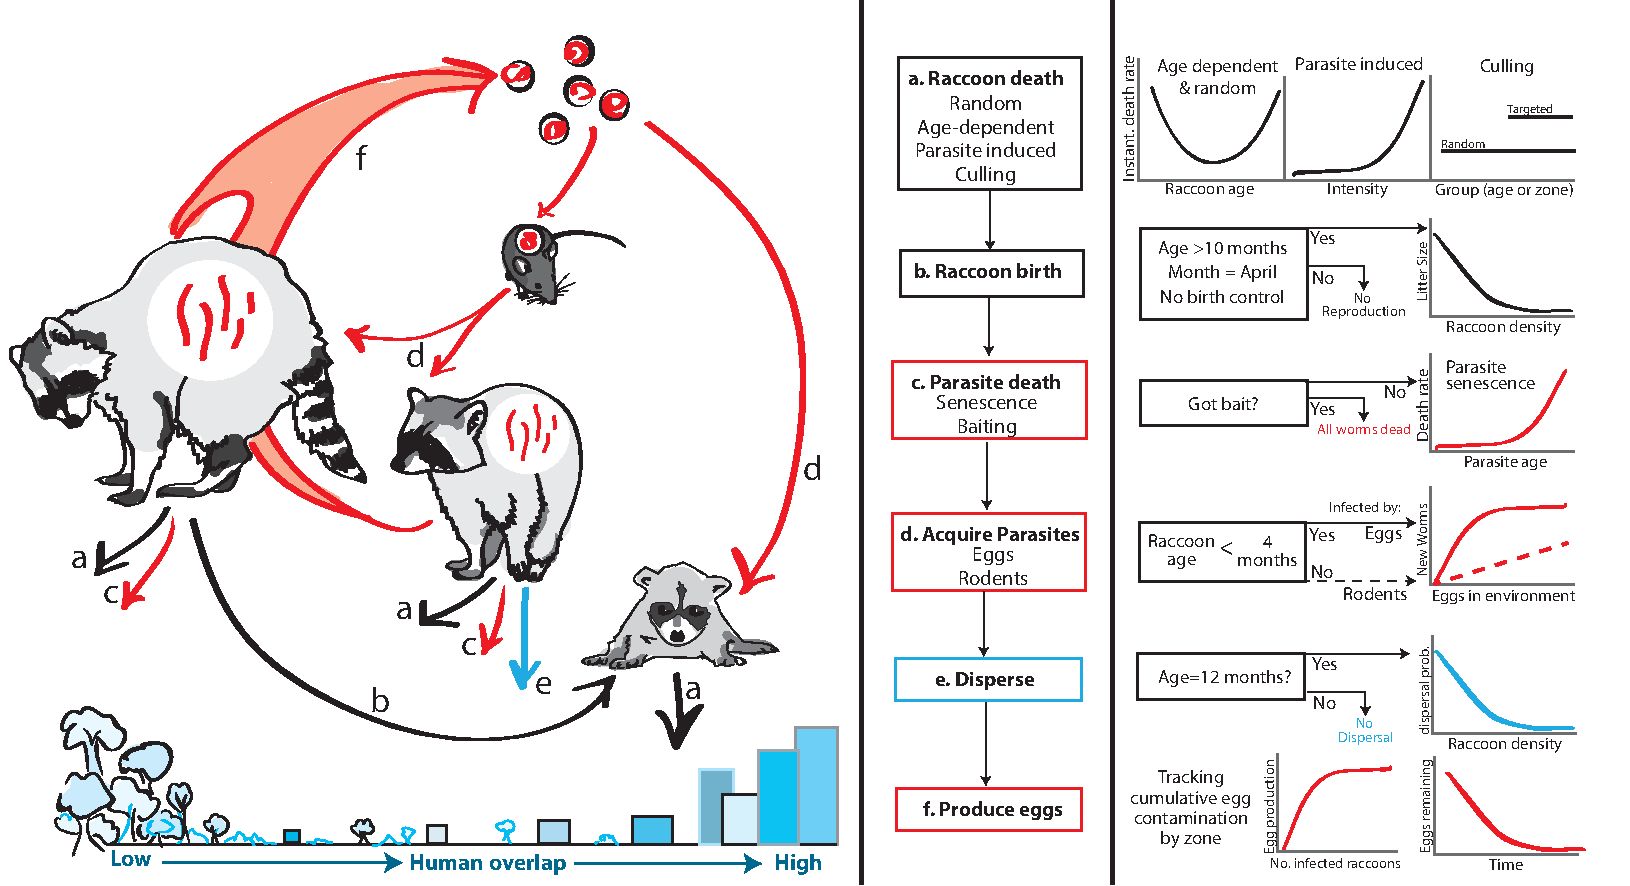
\includegraphics[width=\textwidth]{/Users/mqwilber/Repos/raccoon_simulation/results/plots/lifecycle_model_diagram.pdf}
    \caption{Diagram of the individual-based raccoon-\emph{B. procyonis} model.  The model tracks the raccoons demography (black lines, e.g. age, death, and reproduction), roundworm demography (red lines), and the location of raccoons in the world (blue lines).  In the model, events happen on a monthly time step and can be broken into raccoon-specific (black boxes), worm-specific (red boxes), and location specific (blue boxes) events.}
    \label{fig:mod_diagram}
\end{figure}


\end{document}